\section{Speichern und Audio}

Die Ausgabe der gewünschten Audio-Dateien wird mit einem sogenannten Körperschallaktor umgesetzt welcher in Abbildung \ref*{fig:schallaktorAdafruit} ersichtlich ist. Dieser ermöglicht es, die ausgesendeten Schwingungen über den Schädelknochen weiterzuleiten. Dadurch kann das Mittelohr umgangen werden und die Hygiene verbessert werden, da kein direkter Kontakt mit dem Gehörgang stattfindet. Für den Bau eines Prototyps wird ein Körperschallaktor des Herstellers Adafruit verwendet. 

\begin{figure}[H]
\begin{center}
	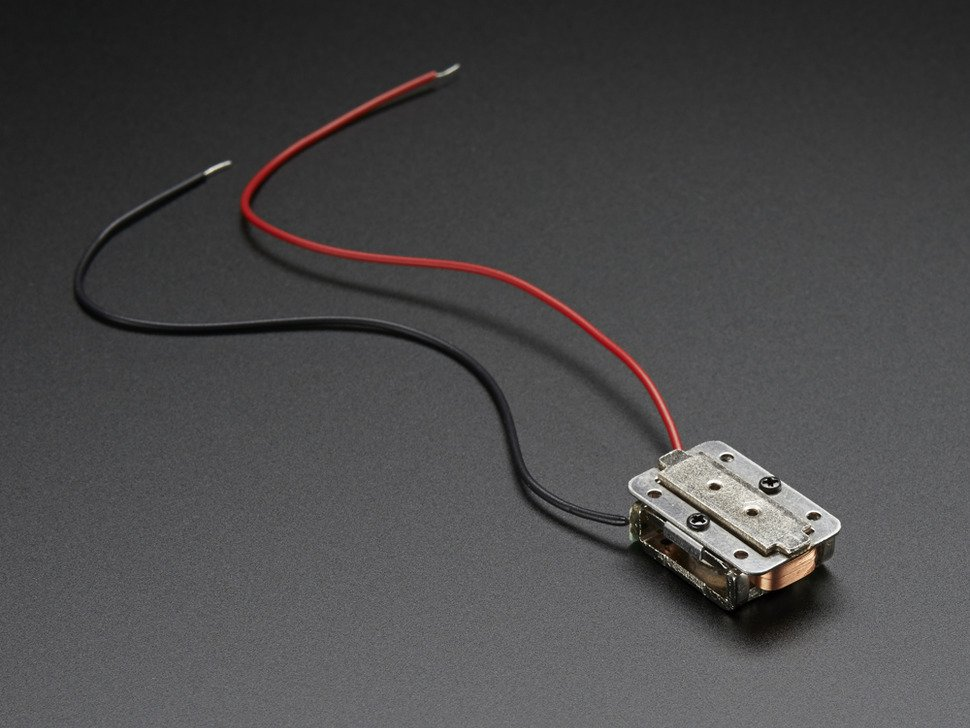
\includegraphics[width=110mm]{data/Schallaktor.png}
	\caption{Körperschallaktor von Adafruit}
	\label{fig:schallaktorAdafruit}
\end{center}
\end{figure}

Das Ziel ist es, bei möglichst geringem Energieverbrauch, eine möglichst intensive Lautstärke, bei guter Audioqualität zu erzielen.
Die Steuerung und Ausgabe der verschiedenen Audiosignale wird von einem zentralen Mikrocontroller übernommen. Ausserdem muss das Audiosignal verstärkt und bei Bedarf gefiltert werden. Damit der Energieverbrauch möglichst gering bleibt, wird die Verstärker und Filterstufe wenn möglich digital durch den Mikrocontroller umgesetzt. Dadurch kann die Anzahl der analogen Bauelemente verringert werden und somit auch der Platzbedarf klein gehalten werden.

Die Speichereinheit wird mit einer externen SD-Karte umgesetzt, die dann manuell entfernt und beschrieben werden kann. Das bedeutet auch, dass die Platzierung der SD-Karte möglichst elegant am Gehäuse erfolgen muss. Alternativ wird versucht den Datentransfer zur Aktualisierung der SD-Karte über die Bluetooth-Verbindung umzusetzen. Die Kommunikation über USB wird vernachlässigt. Damit der Mikrocontroller eine aktive Verbindung zur Speichereinheit hat, wird eine entsprechende Schnittstelle für den Datentransfer zwischen Speichereinheit und Mikrocontroller eingerichtet. Somit kann sich der Mikrocontroller entsprechend der Bluetooth-ID, das jeweils zugehörige Audio-File holen, über die Filter und Verstärkerstufe aufbereiten und anschliessend über den Körperschallaktor ausgeben.
